\section{Global Results}

In the previous section, we analyzed the behavior of a single example. To further interpret the global behavior of the model in the whole dataset, we calculated cross-attention scores and the difference between self-attention and cross-attention vectors for all samples of the test set that were correctly translated (714 samples, \~81\% of the test set), as discussing a false explanation would be meaningless from an epistemological standpoint~\cite{lombrozo2016explanatory,ylikoski2010dissecting}. Then, we averaged them according to the number of glosses per sentence, which allowed us to generate an average visualization for each sentence length, shedding light into the general attention patterns for sentences with a specific number of glosses. These results are illustrated in Figure~\ref{fig:avg_decoder_ca} and Figure~\ref{fig:sa_ca_diff}.

\begin{figure}[htb]
    \centering
    \begin{subfigure}[b]{1.0\textwidth}
        \centering
        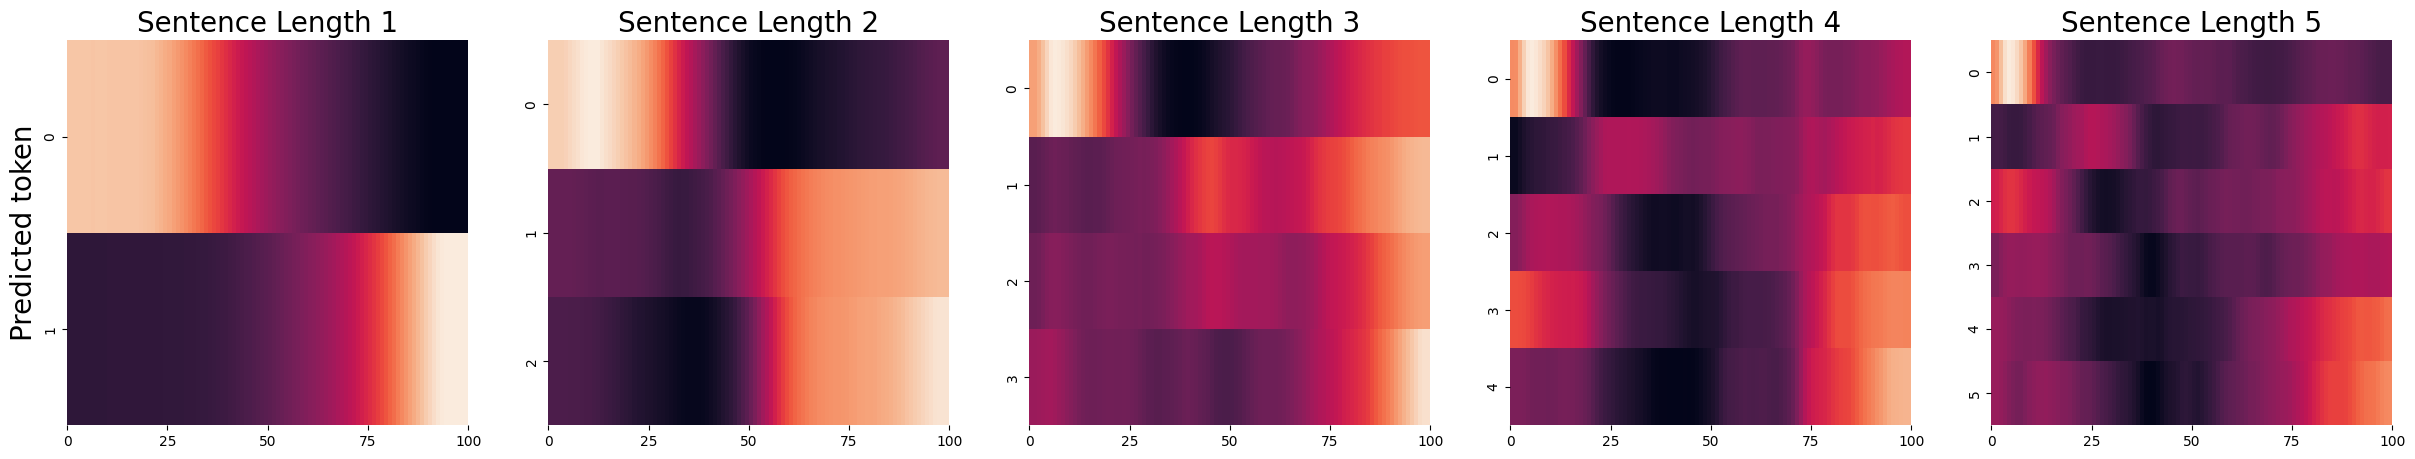
\includegraphics[width=\linewidth]{assets/avg_decoder_ca_1.png}
        \caption{Cross-attention scores for sentences with 1 to 5 glosses, demonstrating a clear and consistent alignment between glosses and clusters of frames.}
        \label{subfig:avg_decoder_ca_1}
    \end{subfigure}\hfill
    \begin{subfigure}[b]{1.0\textwidth}
        \centering
        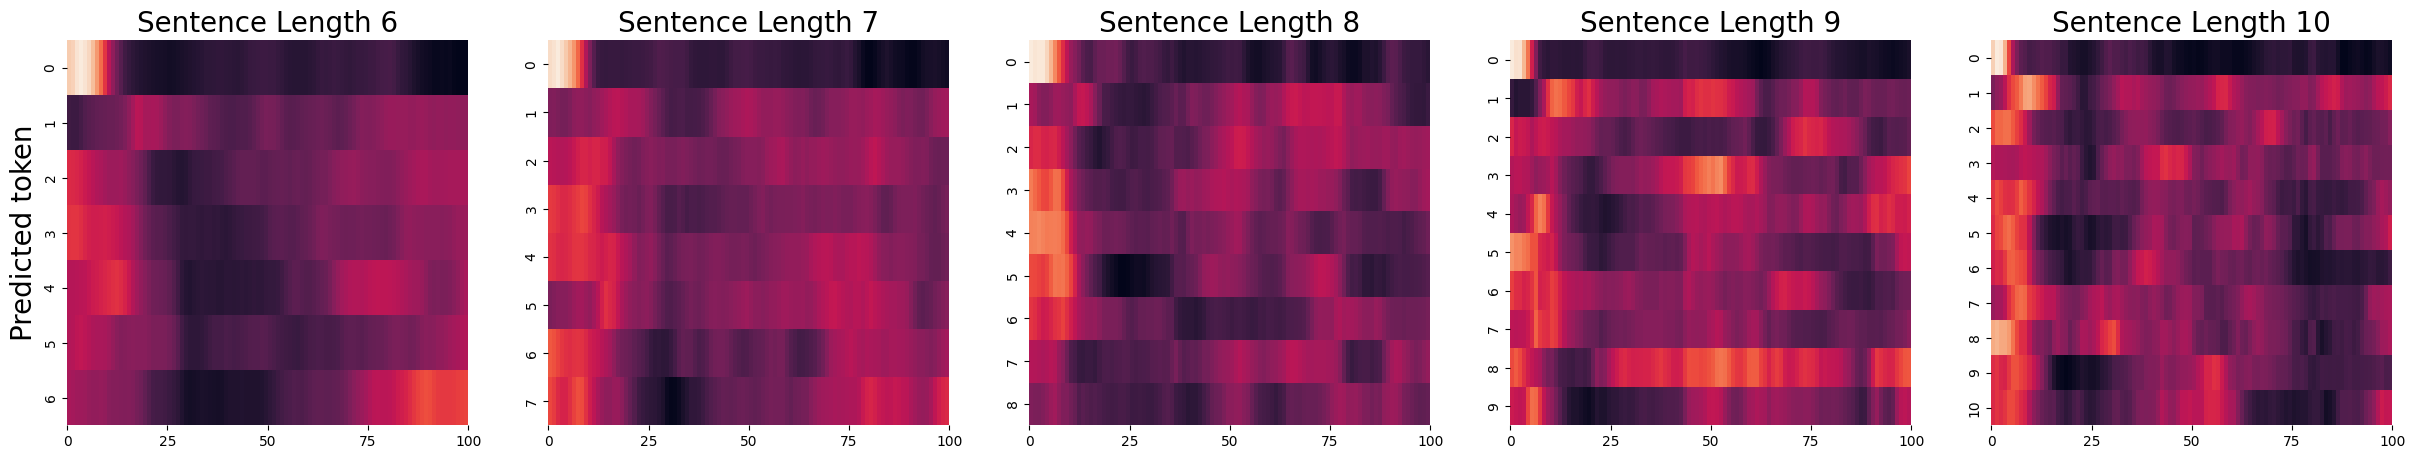
\includegraphics[width=\linewidth]{assets/avg_decoder_ca_2.png}
        \caption{Cross-attention scores for sentences with 6 to 10 glosses. The alignment becomes less distinct, resulting in a more distributed attention pattern across frames.}
        \label{subfig:avg_decoder_ca_2}
    \end{subfigure}
    \caption{\textbf{Average decoder cross-attention scores for different sentence lengths.} Length of the attention weights was normalized to 100.}
    \label{fig:avg_decoder_ca}
\end{figure}

\begin{figure}[htb]
    \centering
    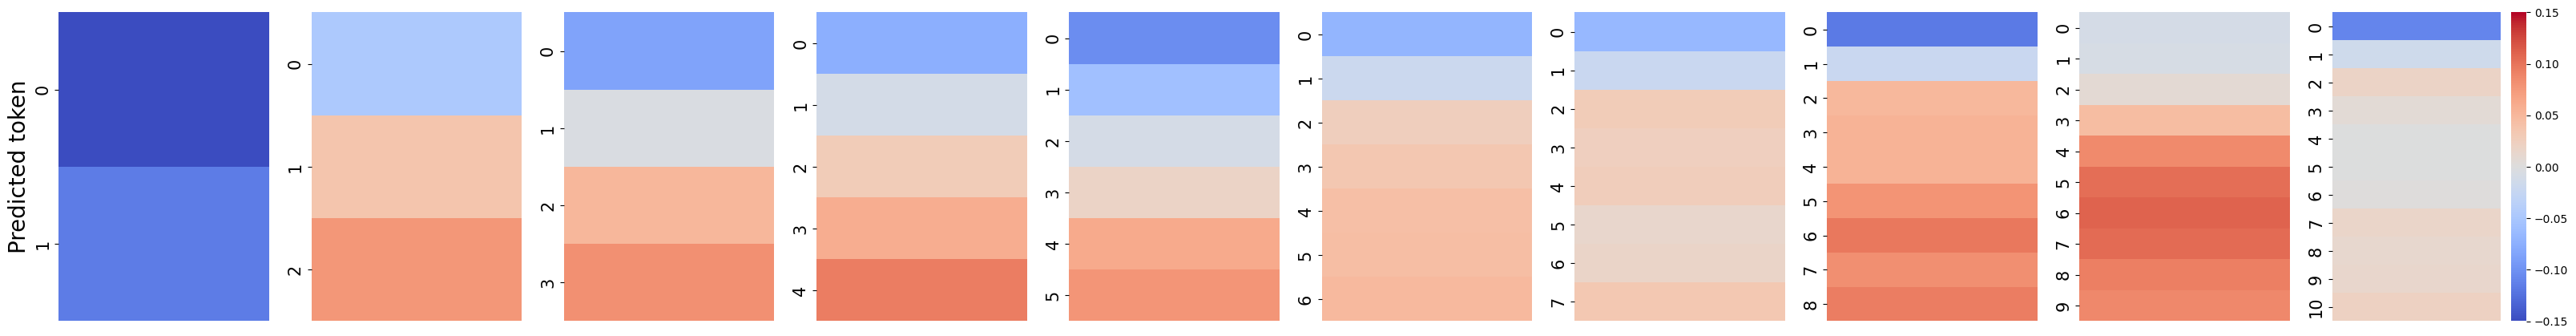
\includegraphics[width=\linewidth]{assets/sa_ca_diff.png}
    \caption{\textbf{Average differences between self-attention and cross-attention for different sentence lengths.}}
    \label{fig:sa_ca_diff}
\end{figure}

% \begin{figure}[htb]
%     \centering
%     \begin{subfigure}[b]{1.0\textwidth}
%         \centering
%         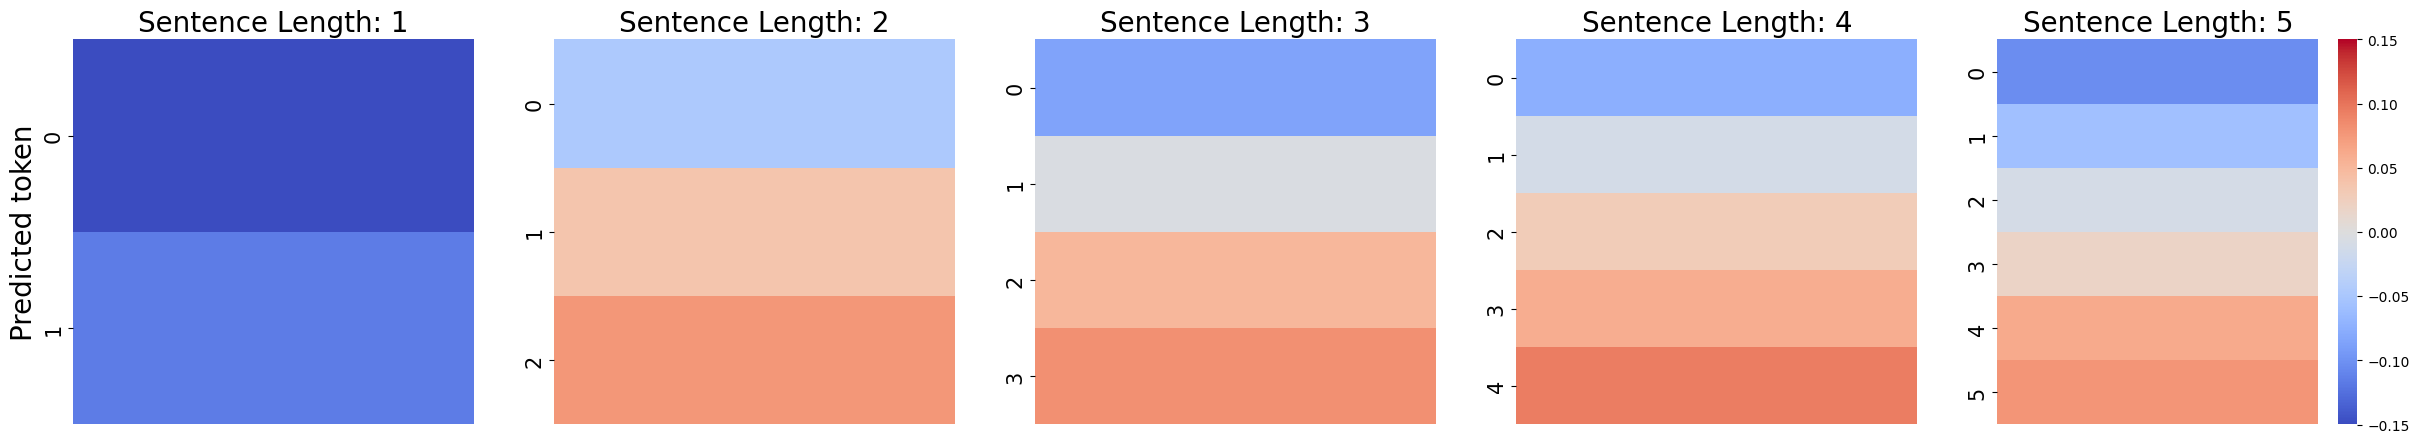
\includegraphics[width=\linewidth]{assets/sa_ca_diff_1.png}
%         \caption{Differences between self-attention and cross-attention for sentences with 1 to 5 glosses. Figure shows a monotonically increasing pattern in self-attention's contribution relative to cross-attention as the number of glosses increases.}
%         \label{subfig:sa_ca_diff_1}
%     \end{subfigure}\hfill
%     \begin{subfigure}[b]{1.0\textwidth}
%         \centering
%         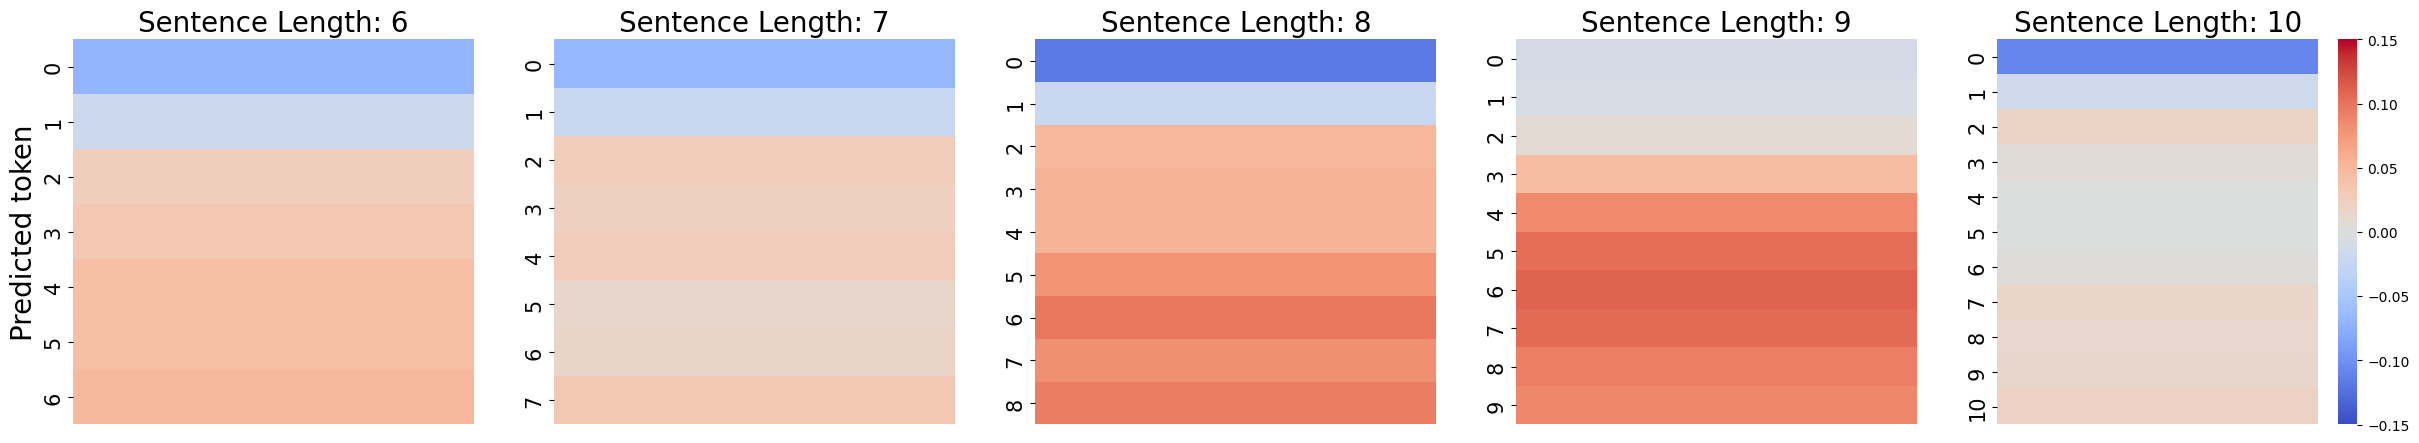
\includegraphics[width=\linewidth]{assets/sa_ca_diff_2.png}
%         \caption{Differences between self-attention and cross-attention for sentences with 6 to 10 glosses. While the figure also shows negative values for initial tokens, self-attention's contribution results dominant as for most of the sequence.}
%         \label{subfig:sa_ca_diff_1}
%     \end{subfigure}
%     \caption{\textbf{Average differences between self and cross-attention contributions when doing inference for each token.}}
%     \label{fig:sa_ca_diff}
% \end{figure}

For sentences containing up to 5 tokens, global results reveal a consistent pattern across the dataset, confirming what was observed from individual examples: 

\begin{enumerate}
    
    \item Cross-attention focuses on clusters of frames than can be mapped to the execution of a whole sign, rather than individual frames.

    \item The attention between poses and glosses aligns in a pattern resembling a diagonal matrix. This suggests that at each decoder step, the model effectively leverages the poses that correspond sequentially with the glosses, demonstrating a clear relationship between specific glosses and associated pose groups

    \item The relevance of the self-attention scores over cross-attention scores monotonically increases alongside the decoder step.
    
\end{enumerate}

However, these patterns become less pronounced as the number of glosses increases. This can be due to several reasons: As more signs are performed per video, and given that the duration of each sign per frame is variable, it is expected for later signs to appear in wider ranges of the video. Also, when more tokens are available, after initially focusing on frames, the model can rely mostly on tokens and use little to no information from the video. In effect, the model is able to predict the whole sentence without the need of identifying individual signs. The fact that in sentences with 8 and 9 glosses, only the first and second rows —where cross-attention dominates over self-attention— retain a semblance of the earlier diagonal pattern, supports   this hypothesis. Finally, it is important to highlight also that there is a significant difference in the amount and variety of examples per sequence length: 84\% of the dataset is composed of 201 different sentences of less than 6 glosses, while videos with 7 or more glosses constitute only 16\% of the dataset and contain 47 different sentences. Having a smaller set of possible target sentences might allow the model to translate the complete sentence with little information from the video, without relying on identifying individual signs.

\subsection{Experiment variants}\label{subsec:variations}

\subsubsection{Embedding size and encoder visualization}

As shown in Table \ref{tab:results}, the size of the hidden dimension did not have a significant impact on its accuracy; however, it did have an impact in terms of interpretability. The patterns described in this work were not found for larger sizes of the hidden dimension. A possible explanation is that, as the hidden dimension sets the size of the representation of each frame generated by the encoder, larger representations allow the encoder to store information about the whole video in a few frames. Figure \ref{fig:avg_encoder_sa} appears to support this hypothesis. The encoder self-attention scores of the 16-dimensions model seem to be distributed along all the frames, seemingly forming as many different patterns as the number of signs in the sentences. On the other hand, for the 32-dimension model, in most cases it seems that only the last frames are being activated.

\begin{figure}[htb]
    \centering
    \begin{subfigure}[b]{1.0\textwidth}
        \centering
        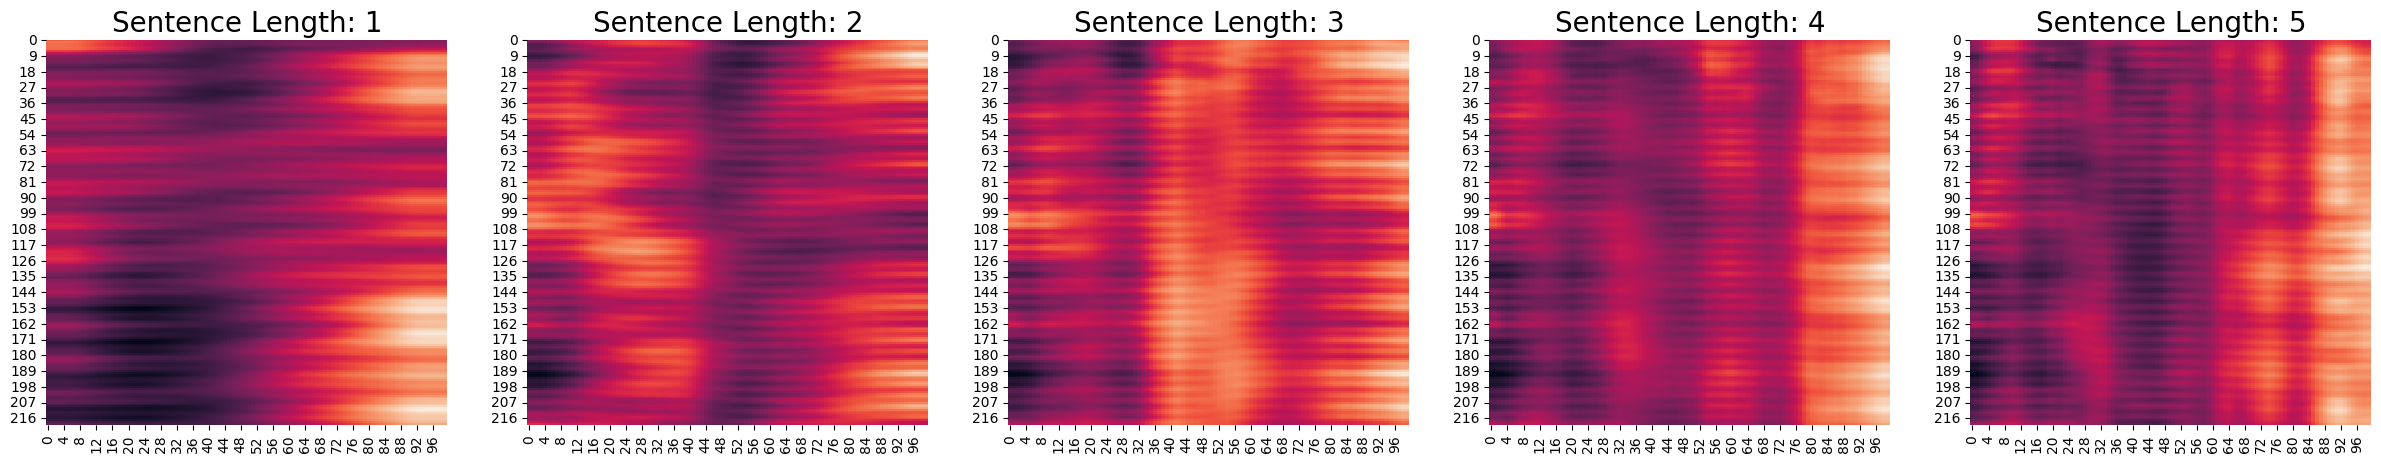
\includegraphics[width=\linewidth]{assets/avg_encoder_sa_16.png}
        \caption{Model with hidden dimension set to 16. This is the same one used for obtaining all other visualizations.}
        \label{subfig:avg_encoder_sa_16}
    \end{subfigure}\hfill
    \begin{subfigure}[b]{1.0\textwidth}
        \centering
        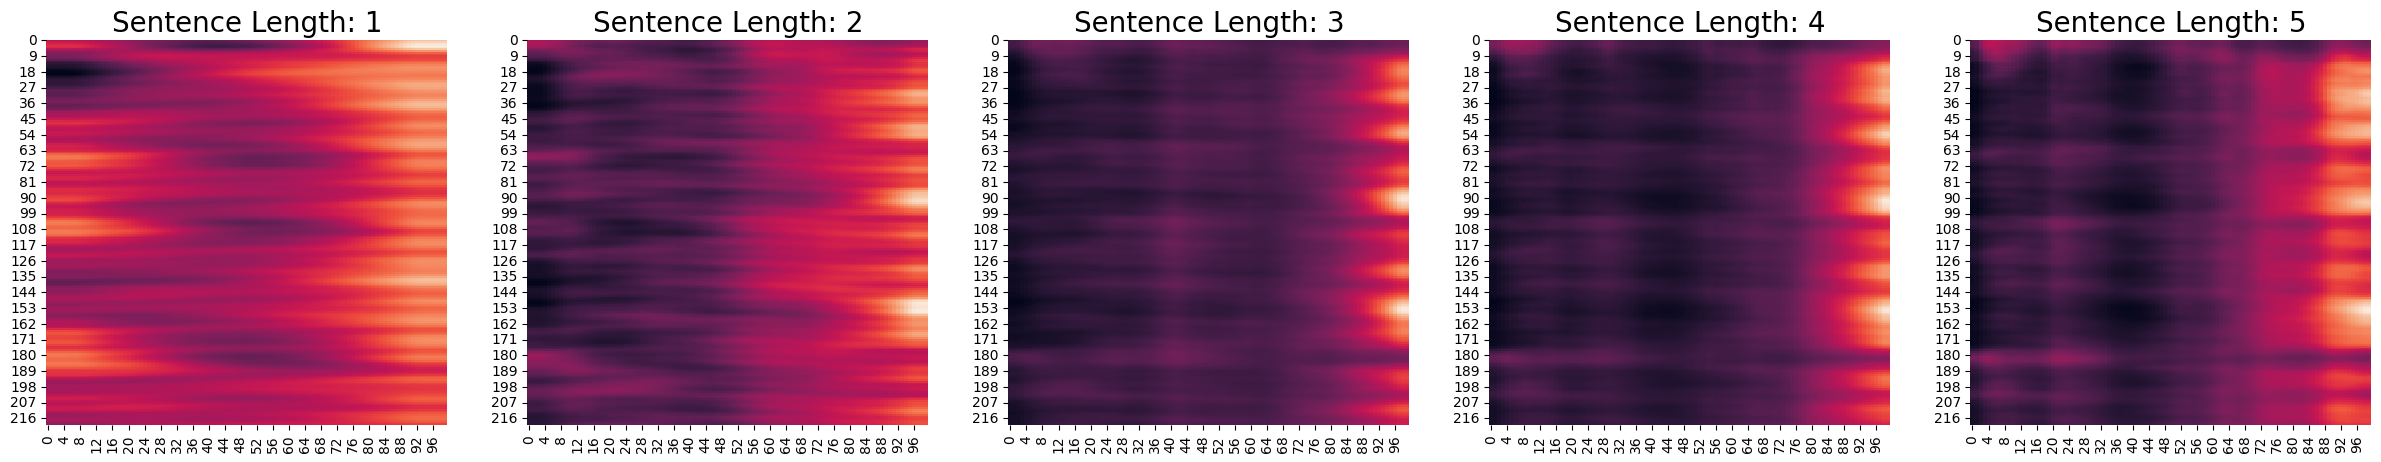
\includegraphics[width=\linewidth]{assets/avg_encoder_sa_32.png}
        \caption{Model with hidden dimension set to 32.}
        \label{subfig:avg_encoder_sa_32}
    \end{subfigure}
    \caption{\textbf{Average encoder self-attention scores for different sentence lengths.} The number of frames was normalized to 100.}
    \label{fig:avg_encoder_sa}
\end{figure}

\subsubsection{Text based model}

We also performed an interpretability analysis on a model that performs proper SLT generating text instead of glosses. The decoder also learned to pay attention to clusters of frames, but these clusters were not diagonally aligned. This is expected due to the grammatical differences and the no one-to-one mapping between written Greek and Greek Sign Language. In addition, cross-attention was more relevant than self-attention for most of the sequence lengths. Figures corresponding to these results can be found in the Appendix.